\documentclass{report}
\usepackage{graphicx}
\usepackage{subcaption}
\usepackage[a4paper, top=0cm, bottom=2cm, left=2cm, right=2cm]{geometry}
\usepackage{titlesec}
\usepackage{fancyhdr}
\usepackage{lipsum} % for generating dummy text

% Define a new geometry for the title page
\newgeometry{a4paper, top=2cm, bottom=2cm, left=2cm, right=2cm}
\newenvironment{mystyle}{
	\setlength{\parindent}{0pt} % No paragraph indentation
	\setlength{\parskip}{10pt} % Adjust the vertical space between paragraphs
	\fontsize{12pt}{14pt}\selectfont % Adjust the font size and line spacing
}{
}
\newcommand{\falcon}{%
	\begin{figure}[htbp]
		\centering
		\begin{subfigure}{0.45\textwidth}
			\centering
			
\includegraphics[width=1\textwidth]{LOGO_ENSAM.png}
		\end{subfigure}
		\begin{subfigure}{0.45\textwidth}
			\centering
			
\includegraphics[width=0.5\textwidth]{Cnesten.jpg}
		\end{subfigure}
		\hrule % Add the horizontal line
	\end{figure}
}

% Configure the fancyhdr package for custom header
\pagestyle{fancy}
\fancyhf{} % Clear header and footer
\renewcommand{\headrulewidth}{0pt} % Remove header rule line
\fancyhead[L]{\falcon} % Set custom header on the left side

% Redefine chapter to avoid page break issues
\let\oldchapter\chapter
\renewcommand{\chapter}[1]{\oldchapter{#1}}

\renewcommand{\theequation}{\arabic{chapter}.\arabic{section}.\arabic{equation}}
\setlength{\parskip}{10pt} % space between paragraphs
% Set line spacing to 1.5
\linespread{1.3}
\begin{document}
	% Apply the title page geometry settings
	\newgeometry{a4paper, top=2cm, bottom=2cm, left=2cm, right=2cm}
	
	\begin{titlepage}
		\falcon        
		\vspace*{2cm}
		
		\centering
		{\LARGE Industrial Project Report \par}
		
		\vspace{1cm}
		
		{\Large Automatique Segmentation of X-ray Images using Deep Learning \par}
		
		\vspace{1.5cm}
		
		{\large Submitted by: \par}
		\vspace{0.5cm}
		
		{\Large DKHISSI SOUFIANE \quad YASSIR BOUSELLAM \par}
		
		
		\vfill
		
		{\large A project submitted in partial fulfillment of the requirements for the degree of \par}
		\vspace{0.5cm}
		
		{\Large Your Degree (e.g., Bachelor's, Master's, etc.) \par}
		
		\vspace{0.5cm}
		
		{\Large GÉNIE INDUSTRIEL: Intelligence Artificielle \& Data Science \par}
		
		\vspace{0.5cm}
		
		{\Large ENSAM Meknes \par}
		
		\vspace{0.5cm}
		
		{\Large 06/09/2023 \par}
	\end{titlepage}
	
	\newpage  % Start on a new page
	
	\section*{}
	\begin{center}
		\huge\textbf{Résumé}
	\end{center}
	
	\vspace{0.5cm} % Adjust the vertical space as needed
	
	
	
	\begin{mystyle} 	Ce compte-rendu de stage d'été, réalisé au sein du Centre National de l'Énergie, des Sciences et des Techniques Nucléaires (CNESTEN), se concentre sur l'utilisation de la Tomographie par Rayons X (XCT) dans le contexte des applications industrielles. La XCT joue un rôle crucial dans le contrôle qualité, la détection des défauts, et l'analyse des défaillances. Notre projet se penche sur un inhalateur de poudre multidose contrôlé par le débit inspiratoire, avec l'objectif de créer un outil de segmentation automatique basé sur l'apprentissage profond.
		
		L'automatisation de l'analyse d'images XCT en trois dimensions dans un environnement industriel est confrontée à des défis complexes. Notre projet vise à évaluer la qualité de l'imagerie dans des situations impliquant des objets composés de matériaux variés, présentant des formes complexes et des propriétés intrinsèques changeantes.
		
		Pour relever ces défis, nous avons opté pour une approche basée sur l'utilisation de plusieurs réseaux neuronaux convolutifs spécialement formés pour traiter des images volumétriques XCT. Afin de préparer notre ensemble de données d'entrée, nous avons effectué une segmentation manuelle, identifiant et classifiant 18 catégories distinctes. Les résultats prometteurs obtenus tant lors de la phase d'entraînement que de la phase de test indiquent la possibilité d'automatiser la segmentation initiale. Tout au long de notre projet, nous avons également exploré des techniques avancées telles que le transfert d'apprentissage et mis en œuvre différents algorithmes d'apprentissage profond pour améliorer notre démarche.
		
		Ce rapport expose les conclusions de notre stage d'été, axé sur la création d'un outil automatisé dédié à l'analyse d'images XCT pour des applications industrielles. Les résultats que nous avons obtenus fournissent des informations précieuses et ouvrent la voie à de futures avancées dans l'exploitation de la tomographie par ordinateur à rayons X (XCT) dans le contexte industriel.
	\end{mystyle}
	
	
	%-------------------------------------introduction-------------------
	%-------------------------------------------------------------------
	\newpage  % Start on a new page
	
	\section*{}
	\vspace{0cm} % Adjust the vertical space as needed
	\begin{center}
		\huge\textbf{Introduction}
	\end{center}
	
	\vspace{1cm} % Adjust the vertical space as needed
	
	
	
	\begin{mystyle} 	Pour garantir la qualité et la conformité de leurs produits, les industriels s'appuient sur des processus d'inspection et d'analyse minutieux. Dans ce contexte, la segmentation automatique des images tomographiques à rayons X (XCT) revêt une importance capitale, permettant une identification et une caractérisation précises des composants des produits.
		
		Cependant, l'inspection manuelle présente des inconvénients, tels que des erreurs potentielles, une subjectivité accrue et des contraintes temporelles. C'est pourquoi notre projet se concentre sur l'automatisation de la segmentation des images XCT. Notre objectif central est de fournir un outil interactif qui simplifie l'utilisation tout en améliorant l'efficacité et la fiabilité des processus d'inspection et de décision.
		
		Nous envisageons d'intégrer des techniques d'apprentissage profond avancées dans une application interactive. Ces techniques, notamment les réseaux de neurones convolutifs (CNN), sont reconnues pour leur capacité à extraire des informations essentielles à partir des images XCT, permettant ainsi une segmentation de haute qualité. Dans notre approche, nous explorerons des architectures de pointe telles que UNet, DeepLabV3, ResNet34, ResNet50, InceptionResNetV2 et 3D U-Net, et évaluerons la performance de chacune de ces architectures.
		
		Cependant, ce qui rend notre démarche unique, c'est notre volonté de créer une solution sur mesure qui s'aligne parfaitement avec les besoins de l'industrie. Nous nous engageons à répondre aux exigences spécifiques de nos partenaires industriels, en adaptant notre application pour correspondre à leurs besoins particuliers.
		
		De plus, nous mettrons l'accent sur l'interface utilisateur de l'application, offrant une expérience conviviale aux utilisateurs finaux en facilitant au maximum la manipulation et la visualisation des modèles. Notre ambition est de simplifier la navigation et l'interaction avec les résultats de la segmentation. Ainsi, les professionnels de l'industrie pourront bénéficier de l'automatisation tout en restant en contrôle total de la solution.
		
		En résumé, notre projet explore l'option d'une application interactive pour la segmentation automatique des images XCT, offrant une expérience utilisateur conviviale tout en améliorant l'efficacité des processus d'inspection et de décision. Notre approche sur mesure et notre engagement envers l'industrie nous permettront de répondre de manière optimale aux besoins spécifiques de nos partenaires tout en offrant des résultats de segmentation de haute qualité.
	\end{mystyle}


\restoregeometry

\renewcommand{\chaptername}{}

\fancyhead[L]{\leftmark \\ \vspace{30pt}}

\chapter{Chapitre I : Présentation de l’organisme d’accueil}

\section{L'organisme et son secteur d'activité }

	\begin{center} % Center the image
		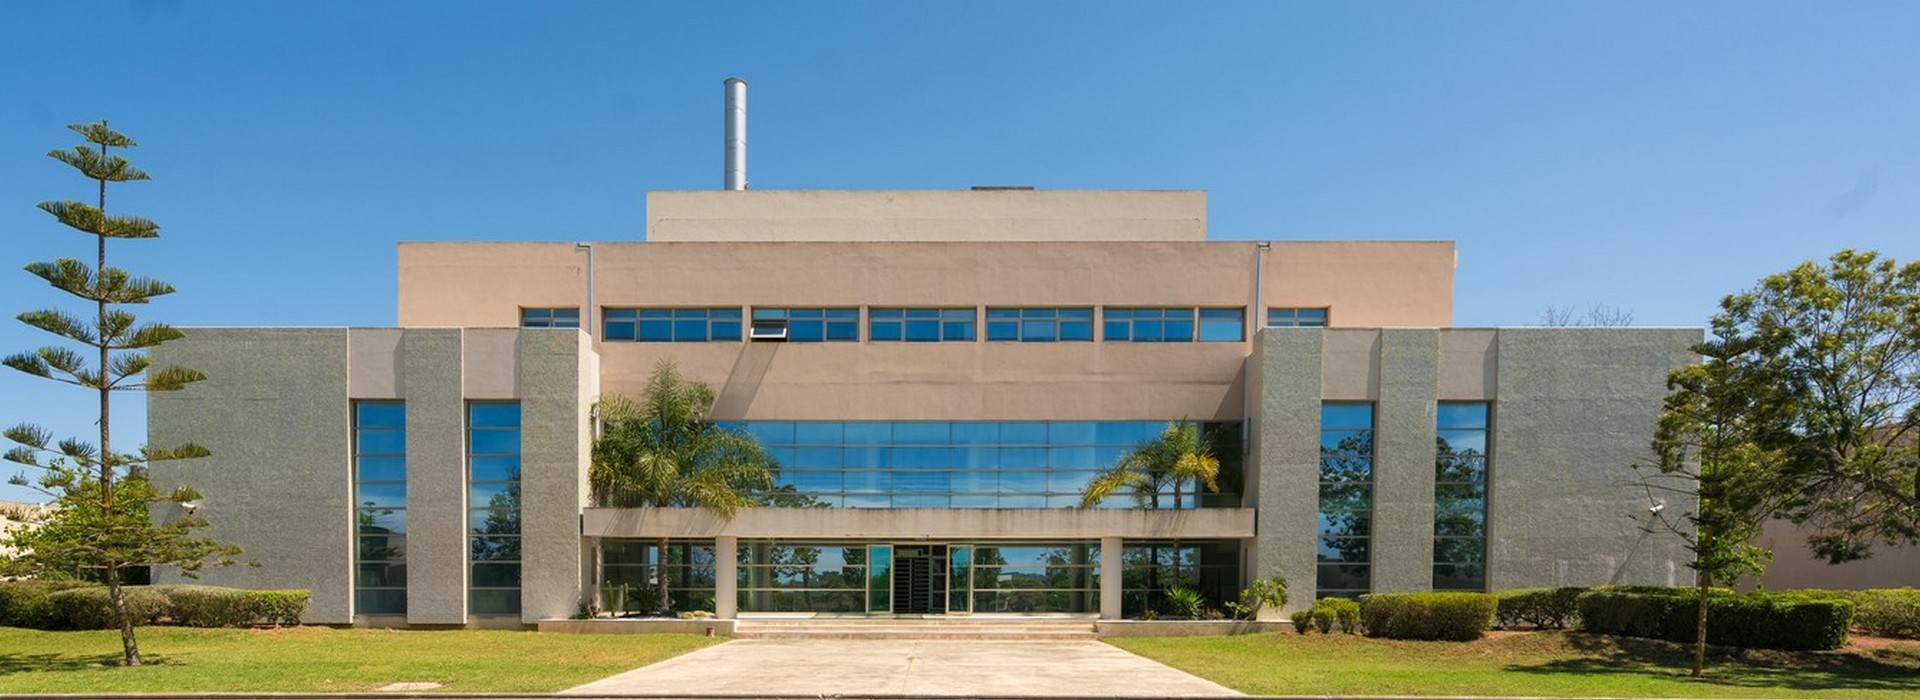
\includegraphics[width=1\textwidth]{space.jpeg} 
		\captionof{figure}{Centre d'études nucléaires de la Maâmoura (CENM).} 
	\end{center}
		\begin{mystyle}  	Le Centre National de l’Energie, des Sciences et des Techniques Nucléaires (CNESTEN) est un établissement public qui a vu le jour grâce au Dahir n° 1-85-98 du 11 Rebia I 1407 (14 novembre 1986), portant promulgation de la loi n° 17-83. Le CNESTEN relève de la tutelle du ministère de la transition énergétique et du Développement Durable, et il occupe une place prépondérante dans le paysage scientifique et technologique du Maroc.
		
		Implanté au Centre d’Etudes Nucléaires de la Maâmora (CENM), qui s'étend sur un vaste site de 25 hectares situé à une trentaine de kilomètres au Nord de Rabat, le CNESTEN dispose d'une infrastructure multidisciplinaire de pointe. La réalisation du CENM a suivi un processus rigoureux d'autorisation conformément au cadre législatif et réglementaire nucléaire national, ainsi qu'aux normes internationales en vigueur.
		
		Au cœur du CENM se trouve un réacteur nucléaire de recherche, constituant un élément central de ses installations. En outre, le centre abrite plusieurs laboratoires et installations spécialisés, dédiés aux différentes applications des sciences et technologies nucléaires. Ces infrastructures sont essentielles pour mener des recherches de pointe, effectuer des analyses approfondies, et contribuer au développement des connaissances et des innovations dans le domaine nucléaire.
		
		Le CNESTEN joue un rôle crucial dans la promotion de l'énergie nucléaire à des fins pacifiques, la recherche scientifique, et la formation de professionnels qualifiés dans le domaine. Il représente un atout majeur pour le Maroc en termes de développement technologique et scientifique dans le secteur nucléaire, contribuant ainsi à la croissance économique et à la sécurité énergétique du pays.
	\end{mystyle}
	
	\section{Réacteur nucléaire de recherche :}
	\begin{center} % Center the image
		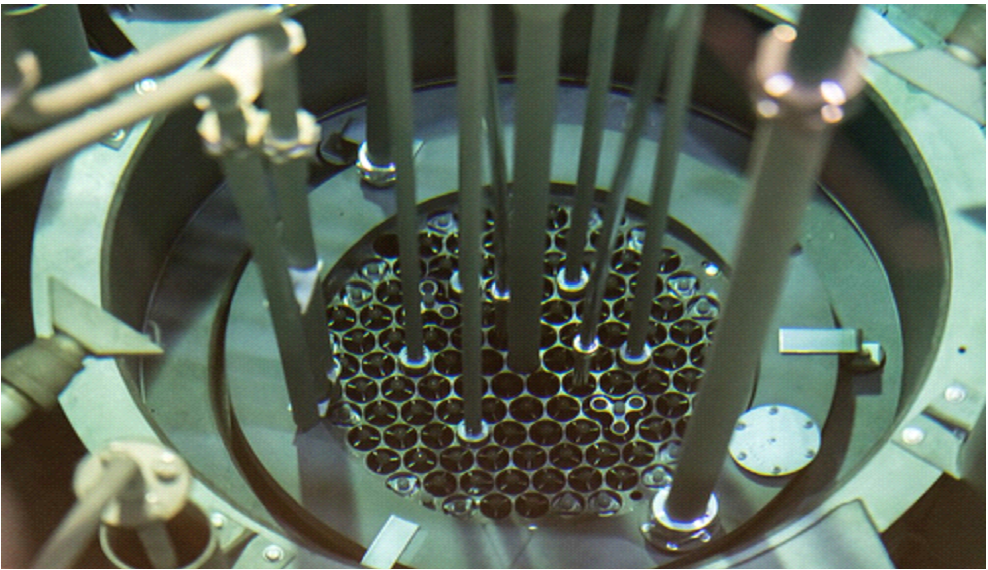
\includegraphics[width=1\textwidth]{reacteur.png} 
		\captionof{figure}{Réacteur TRIGA du CNESTEN} 
	\end{center}
	
	\begin{mystyle} 	L'installation nucléaire unique au Maroc, un réacteur de type TRIGA Mark II d'une puissance nominale de 2MWth, est en exploitation depuis 2009. Ce réacteur nucléaire a été spécifiquement conçu pour répondre à divers besoins et applications dans les domaines de la recherche et de la technologie nucléaires. Il est un atout précieux pour le Centre National de l’Énergie, des Sciences et des Techniques Nucléaires (CNESTEN) et pour le pays dans son ensemble.
	
	Le réacteur TRIGA MARK II du CNESTEN est de conception piscine, ce qui signifie qu'il est situé dans une piscine d'eau. Il utilise l'eau naturelle comme agent de refroidissement, garantissant ainsi un fonctionnement sûr et stable. Ses éléments combustibles sont composés d'hydrure/zirconium-uranium, une configuration qui offre des performances fiables et efficaces.
	
	La gestion du réacteur est assurée par cinq barres de contrôle et trois chaînes neutroniques. Ces dispositifs permettent un contrôle précis de la réaction nucléaire, assurant la sûreté et la sécurité de l'installation.
	
	Le réacteur TRIGA Mark II est polyvalent dans son utilisation. Il est employé pour la production de radio-isotopes, qui sont essentiels dans des applications médicales et industrielles. De plus, il soutient les techniques d'analyses par activation neutronique, l'imagerie et la diffraction neutroniques, des outils cruciaux pour la recherche scientifique et l'analyse des matériaux. Il sert également de plateforme pour la formation de professionnels dans le domaine nucléaire, contribuant ainsi au développement des compétences nationales.
	
	En fin de compte, ce réacteur joue un rôle central dans les programmes du CNESTEN, couvrant une gamme diversifiée de secteurs socioéconomiques, tels que la santé, l'industrie, l'énergie, l'environnement, la géologie, et bien d'autres. Il incarne l'engagement du Maroc envers la promotion de la science et de la technologie nucléaires pour le développement durable et l'amélioration de la qualité de vie de ses citoyens
	\end{mystyle}
	
	\section{Installation de production des Radiopharmaceutiques :}
	
	\begin{mystyle}
		Le CNESTEN dispose d’une installation de production des radiopharmaceutiques, conçue et réalisée conformément aux exigences des bonnes pratiques de fabrication pharmaceutiques et aux exigences de sûreté et de sécurité radiologiques. Cette installation comporte :
		\begin{itemize}
			\item Deux chaînes de cellules chaudes dédiées à la production des radiopharmaceutiques les plus utilisés dans les services de médecine nucléaire au Maroc, à savoir l’iode-131 et les générateurs de Tc-99m .
			\item Une salle blanche pour la production des kits froids.
			\item Et des laboratoires de contrôle qualité.
		\end{itemize}
	\end{mystyle}
	
	\section{Infrastructure de gestion des déchets radioactifs :}
	
	\begin{mystyle}
		Le CNESTEN conformément à sa loi de création de 1986 est désigné comme l’organisme responsable de la gestion des déchets radioactifs générés à l’échelle nationale par les différents opérateurs socio-économiques œuvrant dans les secteurs de la santé, l’industrie, l’agriculture, les mines et la recherche scientifique. Afin de remplir cette mission, le CNESTEN dispose de deux installations pour :
		\begin{itemize}
			\item Le traitement des effluents liquides, le conditionnement des déchets solides, ainsi que le démantèlement des sources radioactives scellées de catégories 3 à 5.
			
			\item L’entreposage de déchets radioactifs conditionnés dans 4 alvéoles, pouvant répondre aux besoins nationaux pour une période d’au moins une trentaine d’années.
			\item Et des laboratoires de contrôle qualité.
				\begin{center} % Center the image
				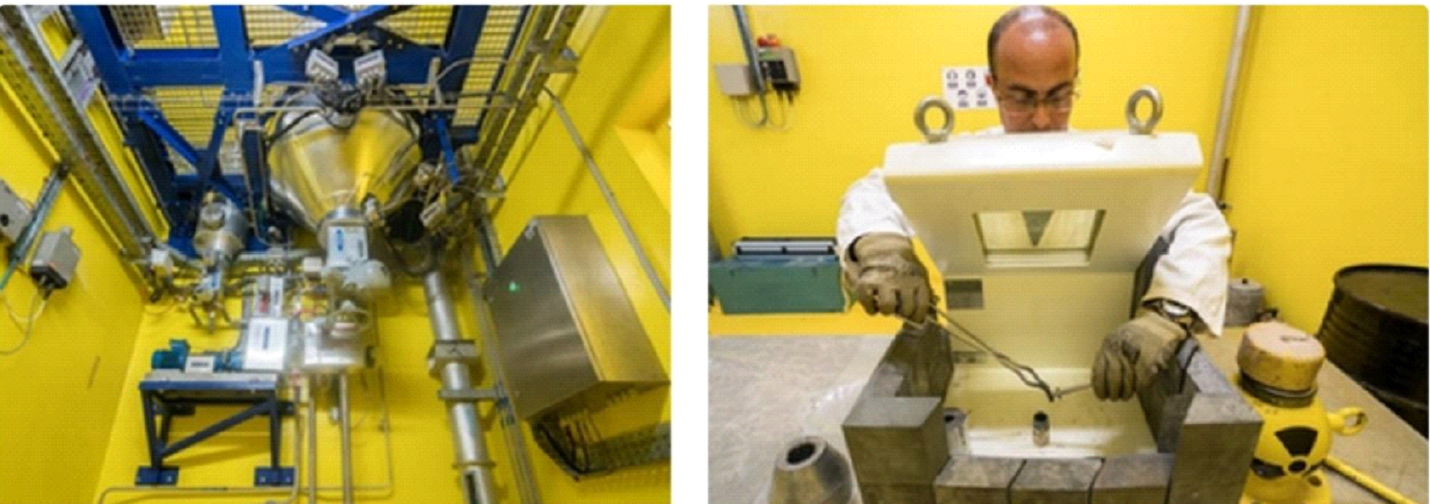
\includegraphics[width=1\textwidth]{yellow.png} 
				\captionof{figure}{Infrastructure de Gestion des Déchets Radioactifs} 
			\end{center}
		\end{itemize}
	\end{mystyle}
	
		\section{Laboratoires :}
	
	\begin{mystyle}
		Le CNESTEN dispose d’un ensemble de laboratoires :
		\begin{itemize}
			\item Laboratoire de contrôle par Radiographie (rayons X et gamma).
			
			\item Laboratoires d’interprétation des radiogrammes.
			\item Laboratoire de contrôle par ressuage et Magnétoscopie : chaîne de ressuage post émulsifiant, bans de magnétoscopie direct et indirect.
			\item Laboratoire de contrôle par Ultrasons.
			\item Laboratoire Jauges et Traceurs : système de tomographie par rayons Gamma, Jauge Neutron Back Scattering, Jauge de turbidité à rayons X pour les études des sédiments en suspension.
			\begin{center} % Center the image
				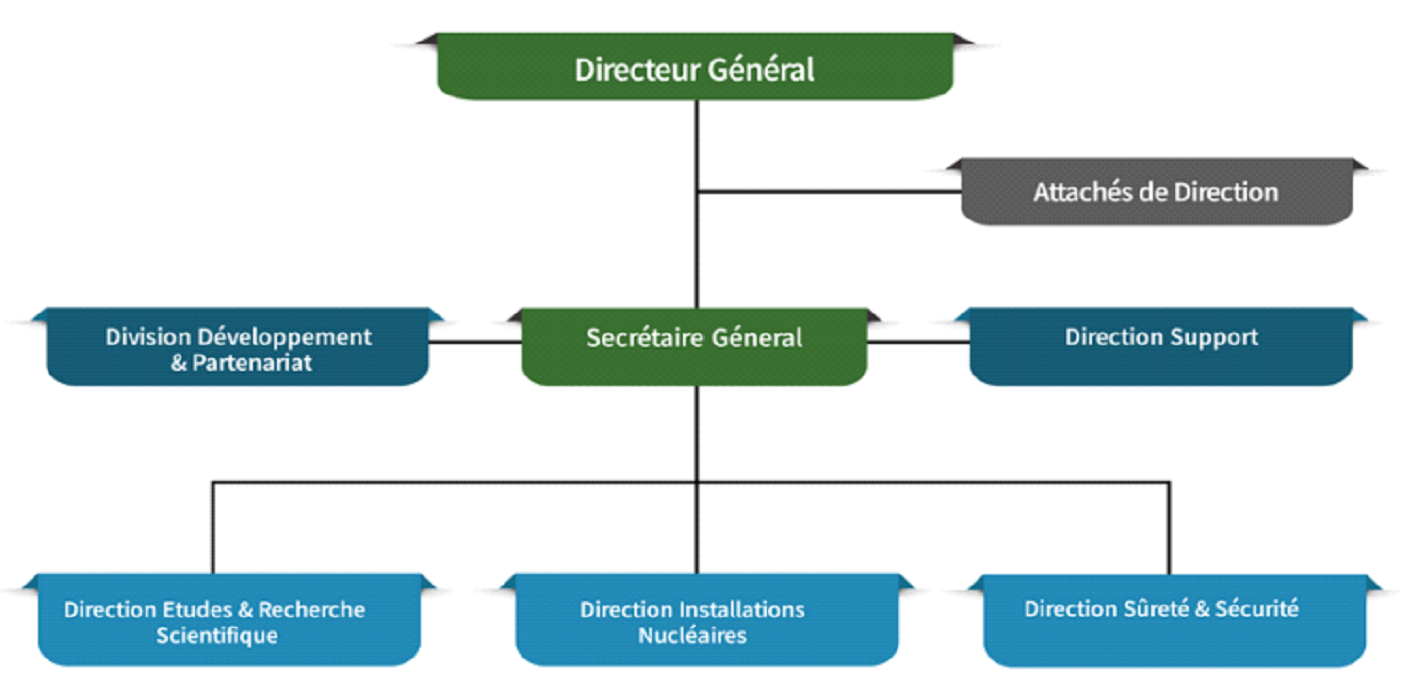
\includegraphics[width=1\textwidth]{organisme.png} 
				\captionof{figure}{organigramme(Cnesten)} 
			\end{center}
		\end{itemize}
	\end{mystyle}
	
	
			\section{Missions et Objectifs de l’organisme}
	
	\begin{mystyle}
		Les missions qui sont imparties au CNESTEN s’articulent autour de : 
		\begin{itemize}
			\item La Promotion de la recherche scientifique et des applications nucléaires dans les secteurs socioéconomiques.
			
			\item La contribution à la préparation des bases technologiques pour un programme électronucléaire.
			\item  L’appui technique aux autorités dans les domaines de la sûreté et la sécurité nucléaires et radiologiques, ainsi que la préparation et la réponse aux situations d’urgences.
			
			\item La gestion des déchets radioactifs au niveau national. Ces missions confient au CNESTEN une triple vocation : centre de recherche, conseil et appui technique aux autorités et prestataire de service.

		\end{itemize}
		
		\begin{center} % Center the image
			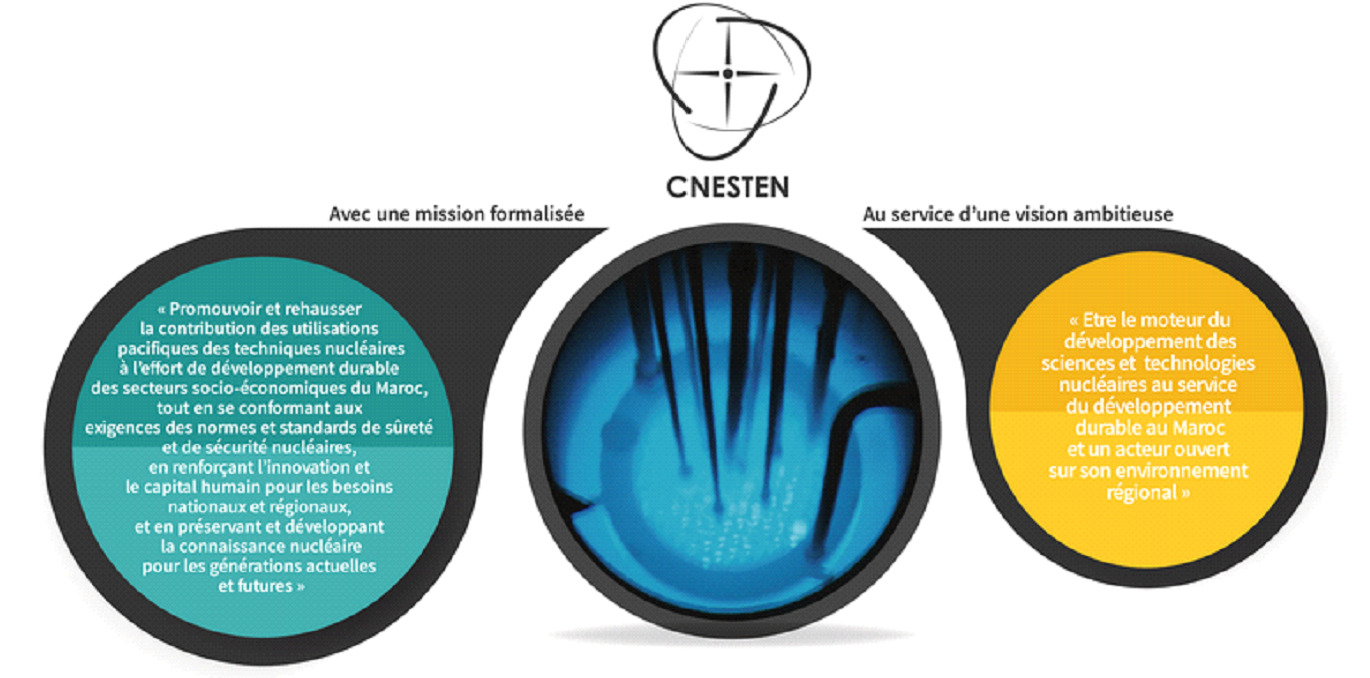
\includegraphics[width=1\textwidth]{triplet.png} 
			\captionof{figure}{Triple vocation)} 
		\end{center}
		Le CNESTEN s’est fixé les objectifs stratégiques suivants :
		
		\begin{enumerate}
			\item Renforcer et élargir les utilisations des sciences et techniques nucléaires dans les programmes et stratégies sectoriels. 
			
			\item Enrichir le capital humain national dans le domaine des sciences et technologies nucléaires.
			\item Renforcer le régime opérationnel de sûreté et de sécurité nucléaires et radiologiques à l’échelle nationale.
			\item Asseoir le positionnement du CNESTEN à l’échelle régionale en sciences et technologies nucléaires au service du rayonnement du Royaume.
		\end{enumerate}
	\end{mystyle}
	
	\section{Principales réalisations de l’Unité de Contrôle Non Destructifs (UCND) :}
		\begin{mystyle}
			Le Projet de ce stage   a été réalisé au sein de la Direction Études & Recherche Scientifiques, Division des Applications Industrielles, Unité Contrôle Non-Destructifs, reconnue à l’échelle nationale et internationale par les réalisations suivantes :
		\end{mystyle}
		
	\subsection{A l’échelle national}
		\begin{mystyle}
				\begin{itemize}
					\item Contribution à la mise en place d'un système national de certification des opérateurs en Contrôles Non Destructifs (CND).
					
					\item Établissement d'un centre de formation et d'examen en CND, unique centre agrée par la Confédération Marocaine des Essais Non Destructifs (COMEND) au niveau national.
					
					\item  Formation et/ou certification de plus de 100 opérateurs CND nationaux et étrangers annuellement.
					
					\item Etudes et expertise utilisant les techniques de CND, sources scellées radioactives ou radiotraceurs au profit de divers industrie.
				\end{itemize}
		\end{mystyle}
		
		\subsection{A l’échelle régional}
		\begin{mystyle}
			\begin{itemize}
				\item Le CNESTEN est reconnu par l’Accord AFRA/AIEA (Organisation régionale africaine de la propriété intellectuelle/Agence internationale de l'énergie atomique) comme un Centre d’Excellence Régional en Contrôle Non Destructif.
				
				
				\item Dans le cadre de la coopération avec l’AIEA et AFRA, le CNESTEN contribue au renforcement des capacités africaines en CND et jauges et traceurs, à travers la formation/certification, l’expertise et les prestations.   
			\end{itemize}
		\end{mystyle}
		\section{Conclusion}
				\begin{mystyle}
					En somme, le Centre National de l'Energie, des Sciences et des Techniques Nucléaires (CNESTEN) occupe une place centrale et essentielle dans le paysage des sciences et technologies nucléaires au Maroc. Grâce à ses installations de pointe, ses missions variées et ses réalisations impressionnantes, le CNESTEN s'affirme comme un acteur de premier plan dans la promotion et l'application des sciences nucléaires dans divers secteurs socioéconomiques. Le prochain chapitre contextualisera davantage le projet en expliquant les motivations sous-jacentes ainsi que les objectifs qui ont orienté sa réalisation. Cette étape permettra de mieux comprendre l'importance et la pertinence de cette initiative dans le cadre des activités du CNESTEN et de son impact potentiel sur le développement du pays.
		\end{mystyle}
		\chapter{Chapitre II : Contexte du projet}
		
		\section{Cadre générale du projet}
		\begin{mystyle}
			Dans le contexte global de notre projet, notre objectif principal consiste à mener des recherches et à développer un outil innovant basé sur les techniques de deep learning, avec pour ambition de révolutionner le contrôle et l'inspection de pièces industrielles en termes de qualité, notamment dans le domaine du Contrôle Non Destructif (CND).
			
			L'inspection manuelle, bien qu'elle ait été le socle de nombreuses industries pendant des décennies, présente des limites considérables, notamment en termes d'efficacité, de subjectivité et d'incertitude associée aux résultats. C'est dans ce contexte que l'utilisation d'images XCT (tomographie par ordinateur à rayons X) se révèle particulièrement pertinente, car elle offre des informations tridimensionnelles détaillées sur les pièces industrielles. Cependant, pour tirer pleinement parti de ces images, il est impératif de disposer d'un outil capable de segmenter automatiquement ces données.
			
			La segmentation automatique des images XCT permettra de délimiter et d'identifier de manière précise les différentes composantes et structures présentes dans les images volumétriques. Cette analyse fine et détaillée permettra de déterminer de manière objective les critères d'acceptabilité ou de rejet des produits, contribuant ainsi de manière significative à garantir la qualité et la conformité des produits industriels.
			
			Pour relever ce défi, nous nous appuierons sur des techniques de Deep Learning, en particulier sur les réseaux de neurones convolutifs (CNN), qui ont démontré leur capacité exceptionnelle à extraire des caractéristiques complexes et à accomplir des tâches de segmentation avec une précision remarquable. En capitalisant sur les données tridimensionnelles fournies par les images XCT, nous mettrons en œuvre l'architecture 3D U-Net pour créer un CNN parfaitement adapté à la segmentation des produits industriels.
			
			En somme, notre projet vise à révolutionner l'inspection industrielle en tirant parti des avancées en matière de deep learning, pour une analyse plus précise, objective et efficiente des pièces industrielles, contribuant ainsi à garantir la qualité et la conformité des produits dans un large éventail d'industries.
		\end{mystyle}
		
		\section{Intérêt du projet :}
		\begin{mystyle}
			L'importance de notre projet de segmentation des images XCT pour le contrôle de qualité industrielle est véritablement révolutionnaire. Il offre la possibilité de transformer en profondeur la façon dont l'industrie garantit la qualité de ses produits. En automatisant le processus d'inspection grâce aux techniques avancées de deep learning, nous ouvrons la voie à une inspection plus rapide, plus précise et plus fiable des pièces industrielles. Cette automatisation élimine les erreurs potentielles liées à l'intervention humaine, réduit la subjectivité et assure une constance inébranlable dans les évaluations de qualité.
			
			De plus, notre projet permettra de repousser les limites de la détection de défauts et d'anomalies, en identifiant même les irrégularités les plus subtiles ou complexes. Cela renforce la sécurité des produits, améliore leur durabilité et réduit les risques associés à des défauts non détectés. En fin de compte, cela a un impact considérable sur la satisfaction du client, la réputation de l'entreprise et la réduction des coûts liés aux rappels de produits.
			
			En outre, l'adoption de l'automatisation dans le contrôle de qualité offre la possibilité de libérer les ressources humaines pour des tâches plus créatives et stratégiques, tout en permettant une analyse approfondie et en temps réel des pièces industrielles. Cela ouvre des perspectives d'amélioration continue et d'innovation dans l'industrie, renforçant ainsi sa compétitivité sur le marché mondial.
			
			En somme, notre projet ne se limite pas à une amélioration marginale, mais il apporte une transformation majeure dans le domaine du contrôle de qualité industriel. Il repousse les frontières de la technologie pour offrir des avantages significatifs en termes de qualité, de sécurité, de coûts et de compétitivité, tout en libérant le potentiel créatif des professionnels de l'industrie pour de nouvelles innovations et des améliorations continues.
	\end{mystyle}
	
	\section{Etat des lieux et solutions existantes :}
			\begin{mystyle}
				Les méthodes traditionnelles, telles que l'inspection manuelle et les techniques de filtrage, ont longtemps été les piliers de l'industrie pour le contrôle de qualité, mais elles présentent des limitations importantes en termes de subjectivité, d'efficacité et de sensibilité aux défauts complexes. D'autres approches, basées sur le traitement d'images avancées, notamment la segmentation basée sur la texture et les seuils, ont été utilisées, mais elles montrent souvent des lacunes dans leur capacité à gérer les variations de matériaux et de formes.
				
				Plus récemment, l'adoption de techniques d'apprentissage automatique, notamment les réseaux de neurones convolutionnels (CNN), a gagné en popularité. Les CNN se sont révélés capables d'automatiser la détection et la segmentation des défauts, offrant ainsi une précision accrue. Cependant, leur réussite dépend souvent de la disponibilité de données d'entraînement de haute qualité et de modèles spécifiquement adaptés aux caractéristiques des images XCT.
				
				Simultanément, l'intégration de l'analyse 3D et de l'automatisation a ouvert de nouvelles perspectives pour l'industrie, permettant une inspection plus approfondie des structures internes des pièces industrielles. Des logiciels d'analyse dédiés ont également émergé, facilitant le traitement et la visualisation des données XCT. Cette convergence de technologies avancées offre désormais des possibilités sans précédent pour améliorer la qualité du contrôle de qualité industriel en permettant une détection plus précise et une évaluation plus approfondie des défauts, tout en réduisant la dépendance à l'égard de l'inspection manuelle sujette à des erreurs et de l'analyse traditionnelle limitée.
			\end{mystyle}
	
\end{document}
